\chapter{Introduction} \label{chap:intro}

Over the last decade, Software development had a tremendous impact with increasing customer demand and requirements \cite{article:swdemand:ahmed}. 
So, the developers have come up with different techniques to meet this requirement criteria. 
Similarly, increasing product complexity and ambiguity have a significant impact on software development. 
Early user feedback from potential customers in the industry is crucial for creating successful software products because of the growing market uncertainties and consumers' desire to receive integrated solutions to their issues rather than unique software developments \cite{misc:businessmodels:teece}.
With the increasing complexity of products, it becomes challenging to determine user requirements.
Different people can have overlapping or contradicting opinions. 
And to reduce these risks, there has to be early detection of the user's needs and requirements. 
Giving users a ``partially functioning'' system is the most excellent method to determine their requirements \cite{journal:prototyping:davis}.
This ensures that the developers with high uncertainties in the early product development can validate by testing the underlying assumptions \cite{misc:lean:steve}.

Product owners can use this feedback to validate the most critical assumptions about the software product. 
This validation can be used to decide whether to add, remove or update a feature \cite{article:experiments:lindgren}. 
This process is called as \texttt{Experimentation} or \texttt{Crowdsourcing}.  
There has been an increase in interest in the types of experimentation that can take place in product development. 
Fabijan et al. \cite{paper:controlled:experiemnts} have shown the benefits of controlled experiments in many use cases with incremental product improvement. 
Using a valuable experiment can solve real-world problems, although choosing what to work on shouldn't be a random process. 
Hence, successful experiments offer one or more solutions that you think will benefit users.

Over the last few years, the developers are focusing more on automating the software code rather than coding everything stated in the product requirements \cite{article:prototyping:hoffnagle}.
This approach is formally known as a \texttt{Low-code} or \texttt{No-code} approach.
So, if there are UI (User Interface) prototypes using some prototyping tools, they would be lightweight software instead of some concrete UI.
This helps the product owner develop various prototypes and conduct experiments on the users.
Similarly, if the experiments are designed using this approach, it would save a lot of resources and, at the same time, get formal feedback from the users. 

According to Luqi et al. \cite{paper:prototyping:luqi}, Models are used broadly in prototyping because a model represents or describes the aspects of the systems that cannot be described adequately in a system of interest.
Modeling the system is far more convenient and efficient than the actual development process. 
Moderately accurate models can be created using an iterative approach in software development by getting continuous feedback from the users.

Most often, data is used to measure the success of the experiments by getting significant feedback from the users.
Promising experiments are designed to better some goal or metric. 
A worthwhile product experiment's ``secret ingredient'' is meaningful, actionable consumer feedback regarding the effects of your product experiments.
This can be done using the \texttt{Qualitative and Quantitative} data analysis.
Using a combination of qualitative and quantitative data can improve an evaluation by ensuring that the strengths of another balance the limitations of one type of data.
This will ensure that the knowledge is improved by integrating different ways of understandings.
\begin{figure}[ht]
    \centering
    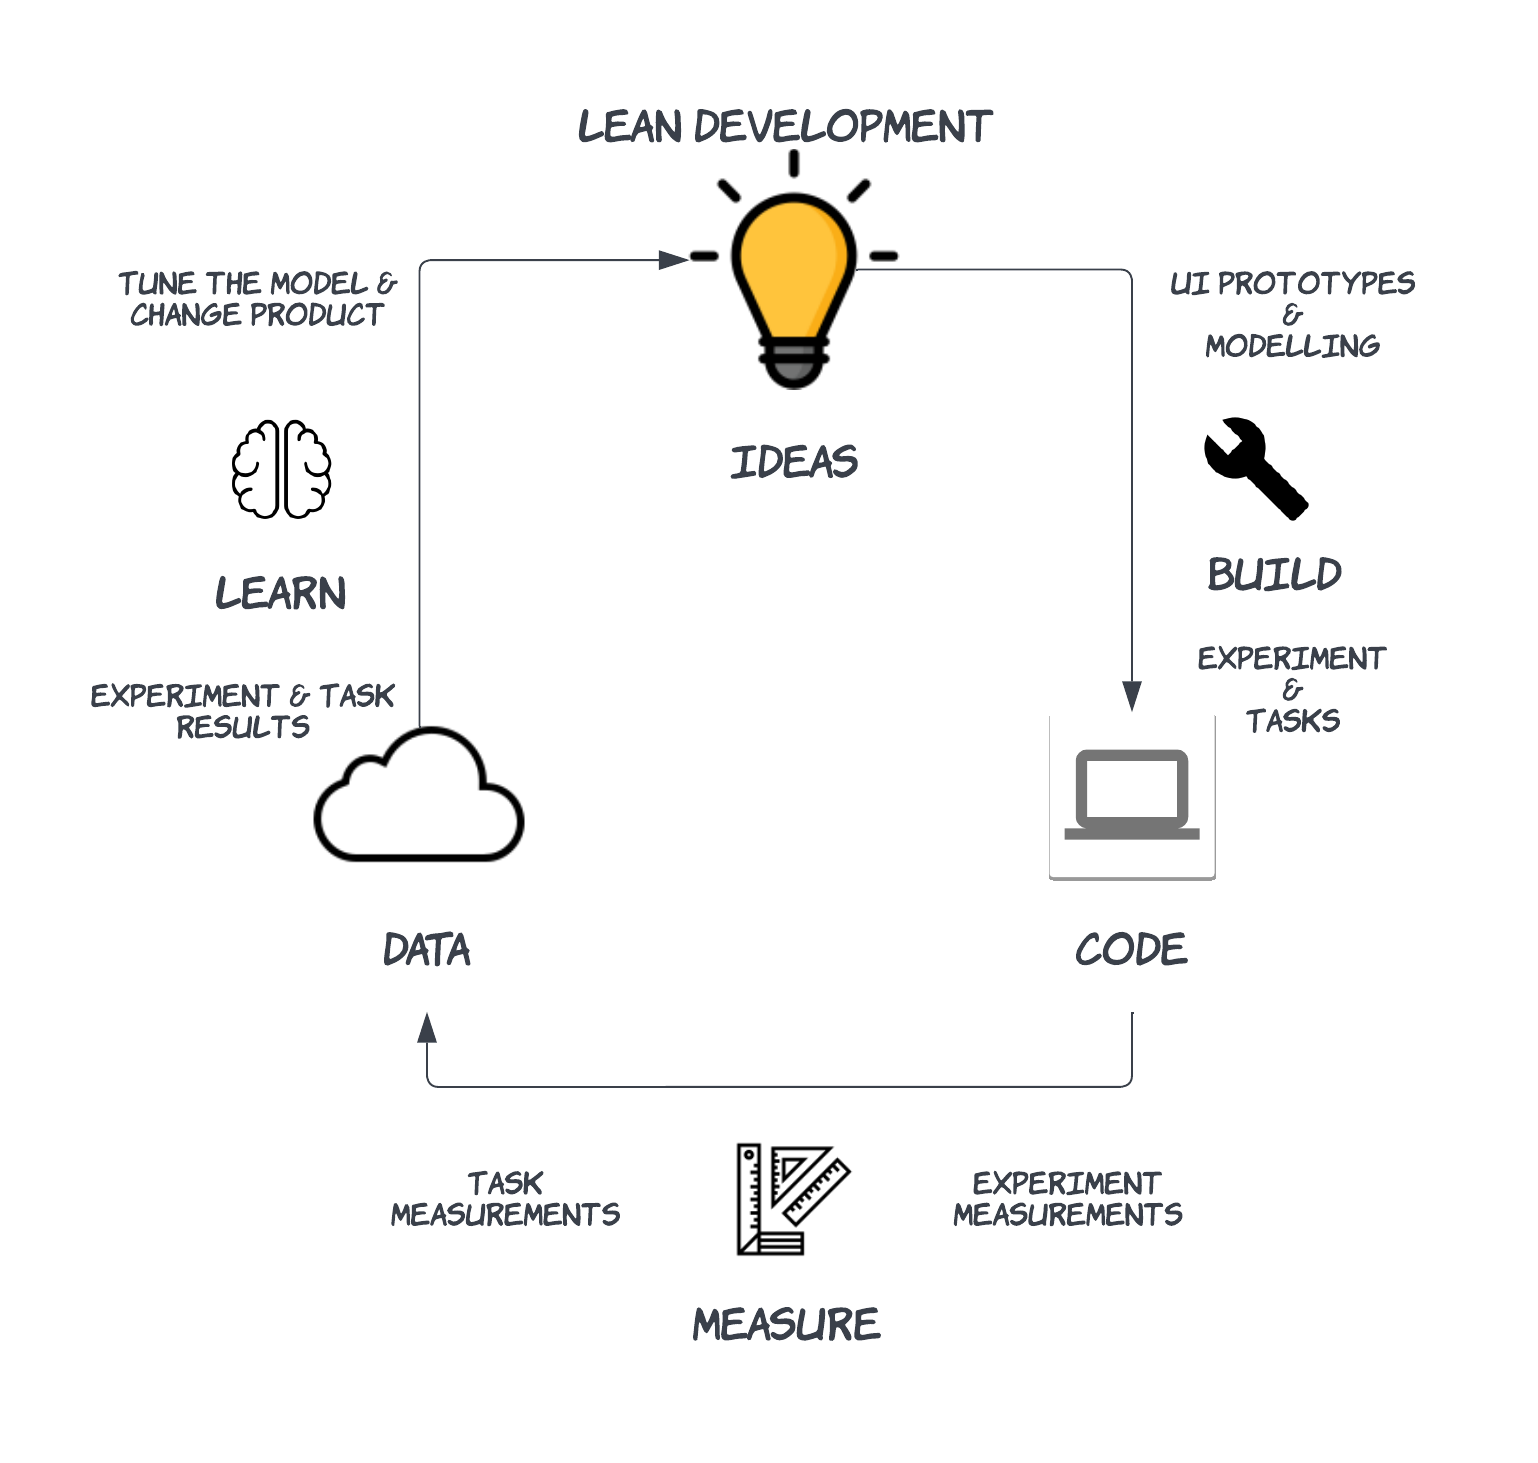
\includegraphics[scale=0.24]{images/solution-ideas/LEAN.png}
    \caption{LEAN Development technique}
    \label{intro:fig:lean}
\end{figure}
\par
In our solution, we propose to combine the model-based and data-driven approaches to solve the problems faced by product owners and developers to have a successful software product.
For that, we use the \emph{LEAN} development technique (see figure \ref{intro:fig:lean}) by starting with \texttt{(1) Ideation and Creating UI prototypes}, then \texttt{(2) Building the product by developing the Models} and using the \texttt{Low-Code technique}, \texttt{(3) Create Experiments} to have a UI for the users and get feedback from the users and finally \texttt{(4) Analyze the data and Tune the model}.